% A good introduction to latex can be found here:
%  http://www.cse.ohio-state.edu/~hank/latex/lshort141.pdf

\documentclass{article}

\usepackage{full page}  % make the margins somewhat smaller than the default

\usepackage{listings}  %  needed for source code listings
\usepackage{color}
\usepackage{graphicx}

\definecolor{javared}{rgb}{0.6,0,0} % for strings
\definecolor{javagreen}{rgb}{0.25,0.5,0.35} % comments
\definecolor{javapurple}{rgb}{0.5,0,0.35} % keywords
\definecolor{javadocblue}{rgb}{0.25,0.35,0.75} % javadoc
 
\lstset{language=Java,
basicstyle=\ttfamily,
keywordstyle=\color{javapurple}\bfseries,
stringstyle=\color{javared},
commentstyle=\color{javagreen},
morecomment=[s][\color{javadocblue}]{/**}{*/},
numbers=left,
numberstyle=\tiny\color{black},
stepnumber=2,
numbersep=10pt,
tabsize=4,
showspaces=false,
showstringspaces=false,
frame=shadowbox,
numbers=left
} 

% set the document title, author, and date here.
%  once set, the \maketitle command (within the document)
%  will display them nicely
\title{Missionaries and Cannibals Solution}
\author{Junjie Guan $<$gjj@cs.dartmouth.edu$>$}

\begin{document}
\maketitle

\section{Introduction}


Considering upper bound of states, we can first compute the total number of states, represented by $(n_m + 1) \times (n_c+1) \times (n_b+1)$, where $n_m, n_c, n_b$ represent the number of missionary, carnibal and boats respectively. Then we can eliminate those logically impossible states, such as all the people on the one side, while all the boat on the other side. Then the upper bound would be $(n_m + 1) \times (n_c+1) \times (n_b+1) - 2$.

We can convert each state of carnibal problem into a code, by using factoring. The only three factors that relate to the state are the numbers of minssionary, carnibals and boats. Assuming the range of the three numbers is $R$, the formula can be described as followed:
$$v = n_m \times R^2 + n_c \times R^1 + n_b \times R^0$$
where the $v$ represents tha encoded value,  Let's say $R = 10$, and the initial state of the problem are $n_m = 3, n_c = 3, n_b = 1$, so that $v = 331$ 

I can use a graph to describe the relationship between different states (for simplicity, I only the major parts of the graph, and demostrate a valid path).

\begin{figure*}[!h]
\centering
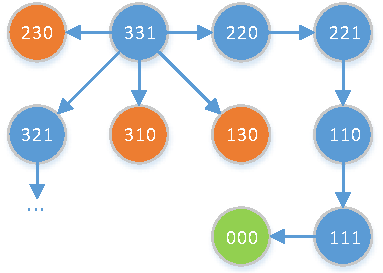
\includegraphics[width=0.618\textwidth]{hw1.pdf}
\caption{A sample graph of states that describe carnibal problem starting with (3, 3, 1), the blue nodes are the normal states, green is the final state, and the orange ones are illegal states.}
\label{states}
\end{figure*}

In Figure \ref{states}, we can see that from a starting states, differnet actions lead to different path, some of them will eventually go to the goal, some of them will run into a dead end.

\section{Implementation of the model}

The model is implemented in 
\verb`CannibalProblem.java`.  Here's my code for \verb`getSuccessors`:

\begin{lstlisting}[numbers=left]
public ArrayList<UUSearchNode> getSuccessors() {
  ArrayList<UUSearchNode> successors = new ArrayList<>();
  // assuming that every time I use as much boat as possible
  if (state[2] != 0) {
    for (int i = 0; i <= Math.min(state[2] * BOAT_SIZE, state[0]); i++) {
      for (int j = 0; j <= Math.min(state[2] * BOAT_SIZE - i,
          state[1]); j++) {
          // make sure the boat is not empty
        if (i + j < totalBoats)	continue;
        CannibalNode tryNode = new CannibalNode(state[0] - i,
            state[1] - j, 0, 0);
        if (isSafeState(tryNode)) {
          successors.add(tryNode);
        }
      }
    }
  } else {
    int state0 = totalMissionaries - state[0], state1 = totalCannibals
        - state[1], state2 = totalBoats - state[2];
    for (int i = 0; i <= Math.min(state2 * BOAT_SIZE, state0); i++) {
      for (int j = 0; j <= Math.min(state2 * BOAT_SIZE - i,
          state1); j++) {
        if (i + j < totalBoats)	continue;
        CannibalNode tryNode = new CannibalNode(state[0] + i,
            state[1] + j, totalBoats, 0);
        if (isSafeState(tryNode)) {
          successors.add(tryNode);
        }
      }
    }
  }
  return successors;
}
\end{lstlisting}

The basic idea of \verb`getSuccessors` is to traverse through every possible state that is contraint by the problem defination (line 6-8) , such as total number of missionary and carnibals, the size of the boat. After getting a new state, it immediately checkes if it is legal (line 11-12). Finally it put the state node into successors list if it is safe.

The order of getting successors is vital to depth first search. I did optimize the codes for DFS, so that during each action it can go to the optimal state, which is transmitting as much people as possible. Simply by replacing line 6-7 as following:

\begin{lstlisting}[numbers=left]
 for (int i = Math.min(state[2] * BOAT_SIZE, state[0]); i >= 0 ; i--) {
   for (int j = Math.min(state[2] * BOAT_SIZE - i,
     state[1]); j >= 0; j--) {
\end{lstlisting}

However, this might lose a lot fun, because by doing so dfs might perform as well as bfs. So I stick to the non-optimized one.

You may find that the \textbf{getSuccessors()} a little verbose. I did try to implement in a more contract way, but it makes the codes more difficult to understand. If you have any short and easy-understand expression, please do tell me.

I used a method called \verb`isSafeState` that returns \verb`true` if the state is legal. Basically it checks the legal state for both side of the river, which is the number of missionsaries should not be less than carnibals'. Or if all the missionaries are at the one side, it is also safe. Here are the codes:

\begin{lstlisting}[numbers=left]
private boolean isSafeState(CannibalNode tryNode) {
  if (tryNode.state[0] == 0 || tryNode.state[0] == totalMissionaries)
    return true;
  else if (tryNode.state[0] >= tryNode.state[1]
      && (totalMissionaries - tryNode.state[0])
      	>= (totalCannibals - tryNode.state[1])
      && tryNode.state[0] >= 0 && tryNode.state[1] >= 0)
    return true;
  else
    return false;
}
\end{lstlisting}

\section{Breadth-first search}

In the following BFS search, I use a queue to keep track of the nodes to be visited. How to determine whether a adjecnt node should be put into the queue? I maintain a hash map for the nodes that have been visited.

Of course the while loop can terminate in two cases, One is when the the current node is the goal, which means we have reached the destination. In this case I use backchrain to build the path. The other is when the queue is empty, which means we've already search the whole connected graph and yet goal is not found. In this case I return null.

\begin{lstlisting}[numbers=left][language=Java]
  public List<UUSearchNode> breadthFirstSearch() {
    resetStats();

    UUSearchNode node;
    HashMap<UUSearchNode, UUSearchNode> visited = new HashMap<>();
    Queue<UUSearchNode> nqueue = new LinkedList<UUSearchNode>();
    List<UUSearchNode> successors;

    nqueue.add(startNode);
    while (!nqueue.isEmpty()) {
      // get node from the queue
      node = nqueue.poll();

      // check if arrives destination
      if (node.goalTest()) {
        updateMemory(visited.size() + 1); // add the start node
        nodesExplored = visited.size() + 1;
        return backchain(node, visited);
      }

      // if not destination, keep searching and tracking
      successors = node.getSuccessors();
      for (UUSearchNode n : successors) {

        if (!visited.containsValue(n)) {
          visited.put(n, node);
          nqueue.add(n);
        }
      }
    }
    // if destination not found, return null
    return null;
  }
\end{lstlisting}

With the input of (3,3,1), the output is as following. The path is in a reverse style:

\begin{lstlisting}[numbers=left]
bfs path length:  12 [0, 111, 10, 31, 20, 221, 110, 311, 300, 321, 220, 331]
Nodes explored during last search:  15
Maximum memory usage during last search 15
Total execution time: 0.6 seconds
\end{lstlisting}

As you can see the path is consistent with my drawing in Figure \ref{states}.

With the input of (8,5,1), the output is as following:

\begin{lstlisting}[numbers=left]
bfs path length:  24 [0, 111, 10, 211, 110, 311, 210, 321, 220, 421, 320,
	431, 330, 531, 430, 541, 440, 641, 540, 651, 550, 751, 650, 851]
Nodes explored during last search:  62
Maximum memory usage during last search 62
\end{lstlisting}













\section{Memoizing depth-first search}

DFS in recursive style is fairly simple, though I am understand why the provided code indicate me to use \textbf{HashMap$<$UUSearchNode, Integer$>$ visited}, while it could be better done by using \textbf{HashSet}. 

\begin{lstlisting}[numbers=left]
public List<UUSearchNode> depthFirstMemoizingSearch(int maxDepth) {
  resetStats();
  HashMap<UUSearchNode, Integer> visited = new HashMap<>();
  return dfsrm(startNode, visited, 0, maxDepth);
}

private List<UUSearchNode> dfsrm(UUSearchNode currentNode,
    HashMap<UUSearchNode, Integer> visited, int depth, int maxDepth) {

  // keep track of stats; these calls charge for the current node
  updateMemory(visited.size());
  incrementNodeCount();

  // you write this method. Comments *must* clearly show the
  // "base case" and "recursive case" that any recursive function has.

  //System.out.println(currentNode);
  List<UUSearchNode> tryPath, path = new ArrayList<UUSearchNode>(
      Arrays.asList(currentNode));
  List<UUSearchNode> successors;

  visited.put(currentNode, depth);
  if (depth > maxDepth)
    return null;      
  
  if (currentNode.goalTest()) {
    return path;
  } else {
    successors = currentNode.getSuccessors();
    for (UUSearchNode n : successors) {
      if(!visited.containsKey(n) || visited.get(n) > depth + 1) {
        tryPath = dfsrm(n, visited, depth + 1, maxDepth);
        if (tryPath != null) {
          path.addAll(tryPath);
          return path;
        }
      }
    }
  }
  return null;
}
\end{lstlisting}

The basic idea is, inside dfs, we run dfs for each legal node, and keep track of each node that have been visited. The trick of using \textbf{HashMap} is, in depth limited search, a node may fail due to the limitation of depth, not because there is a dead end. \textbf{HashMap} keeps tracking of the shortest path to the node, so dfs can find the solution as much as it can.

With the input of (8,5,1), the output is as following:

\begin{lstlisting}[numbers=left]
dfs memoizing path length:34 [851, 830, 841, 820, 831, 630, 641, 540, 551,
  530, 541, 520, 531, 430, 441, 420, 431, 410, 421, 320, 331, 310, 321, 300,
  311, 210, 221, 200, 211, 100, 111, 10, 21, 0]
Nodes explored during last search:  40
Maximum memory usage during last search 39
Total execution time: 0.6 seconds
\end{lstlisting}

As you can see, memorizing dfs use less memory while finding a less optimal path comparing to bfs. Actually in the worth case, when the path is not found until the last try, memorizing dfs uses as much memory as bfs.















\section{Path-checking depth-first search}

\begin{lstlisting}[numbers=left]
public List<UUSearchNode> depthFirstPathCheckingSearch(int maxDepth) {
  resetStats();
  HashSet<UUSearchNode> currentPath = new HashSet<UUSearchNode>();
  return dfsrpc(startNode, currentPath, 0, maxDepth);
}

private List<UUSearchNode> dfsrpc(UUSearchNode currentNode,
    HashSet<UUSearchNode> currentPath, int depth, int maxDepth) {

  // keep track of stats; these calls charge for the current node
  updateMemory(currentPath.size());
  incrementNodeCount();

  List<UUSearchNode> successors, tryPath, path 
  	= new ArrayList<UUSearchNode>(Arrays.asList(currentNode));

  //System.out.println(currentNode);
  if (depth > maxDepth)
    return null;
  else 
    currentPath.add(currentNode);

  // This is base case where search reaches the goal
  if (currentNode.goalTest()) {
    return path;
  } else {
  
    successors = currentNode.getSuccessors();
    for (UUSearchNode n : successors) {
      if (!currentPath.contains(n)) {
        // This is the recursive function
        tryPath = dfsrpc(n, currentPath, depth + 1, maxDepth);
        if (tryPath != null) {
          path.addAll(tryPath);
          return path;
        }
      }
    }
  }
  currentPath.remove(currentNode);
  return null;
}
\end{lstlisting}

The basic idea is similar to memorizing dfs. The only difference is when rolling the path, it marked the node as not visited. We don't have to use \textbf{HashMap} here, because any node being rolled is legal to revisit again.

\begin{figure*}[!h]
\centering
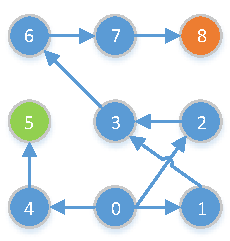
\includegraphics[width=0.5\textwidth]{hw1-fig-2.pdf}
\caption{An example that demostrate difference between memorizing and path-checking dfs}
\label{diff}
\end{figure*}

This may cause some redundance when seacrhing the graph. Take Figure \ref{diff} for example, in memorizing, if we first check $(0 \rightarrow 1 \rightarrow 3 \rightarrow 6 \rightarrow 7 \rightarrow 8)$, and turn out to be dead end. Then we check $(0 \rightarrow 2)$, but we won't go further anymore, since node $3$ is visited. But in path-checking, it probably check $(0 \rightarrow 1 \rightarrow 3 \rightarrow 6 \rightarrow 7 \rightarrow 8)$, $(0 \rightarrow 1 \rightarrow 2 \rightarrow 6 \rightarrow 7 \rightarrow 8)$, and finally $(0 \rightarrow 4 \rightarrow 5)$.

An obvious advantage of path-checking over memorizing is using less memory, the maximum possible memory used is the longest path, which is usually much smaller the size of graph.

With the input of (8,5,1), the output is as following:

\begin{lstlisting}[numbers=left]
dfs path checking path length:34 [851, 830, 841, 820, 831, 630, 641, 540, 551, 530, 541, 520, 531, 430, 441, 420, 431, 410, 421, 320, 331, 310, 321, 300, 311, 210, 221, 200, 211, 100, 111, 10, 21, 0]
Nodes explored during last search:  40
Maximum memory usage during last search 33
Total execution time: 0.6 seconds
\end{lstlisting}













\section{Iterative deepening search}

\begin{lstlisting}[numbers=left]
public List<UUSearchNode> IDSearch(int maxDepth) {
  resetStats();
  HashSet<UUSearchNode> currentPath = new HashSet<UUSearchNode>();
  List<UUSearchNode> path;
  for (int i = 1; i <= maxDepth; i++) {
    currentPath.clear();
    path = dfsrpc(startNode, currentPath, 0, i);
    if (path != null)
      return path;
  }
  return null;
}
\end{lstlisting}

The basic idea is use several path-checking dfs, while gradually increasing the maximun search depth, until we reach the goal. The problem is, should we choose memorizing or path-checking style dfs as the iterative function? Assuming that the graph is complicate enough. In terms of memory, no doubt that path-checking will be very likely use less memory, since memorizing need to store all the visited nodes. While in terms of time, memorizing may safe some time, when there are two path overlap and paht-checking need to re-visit it. But, on the other hand, there are high chances that ids with memorizing dfs performs worse than simply bfs, in terms of both memory (also need to safe a lot of nodes, and also need extra space in the stack for recursive function) and time. So, we might have just well using bfs. In short, there is no strong reason to use memorizing as interative funciton in ids.

With the input of (8,5,1), the output is as following:

\begin{lstlisting}[numbers=left]
Iterative deepening (path checking) path length:24 [851, 830, 841, 820,
  831, 630, 641, 530, 541, 520, 531, 420, 431, 410, 421, 310, 321, 300,
  311, 200, 211, 100, 111, 0]
Nodes explored during last search:  38918999
Maximum memory usage during last search 24
Total execution time: 4.953 seconds
\end{lstlisting}






\section{Lossy missionaries and cannibals}

In this situation, no more than E missionaries can be eaten. Then I can use a new state to describe: $(m, c, b, e)$, where $m, c, b$ is the same as before, $e$ represent whether the missionaries are eatable. I will basically change the conditions in \textbf{isSafe} depends on how many missionaries have already been eaten, if $n_e$ exceeds E, I will set $e = false$, as no more missionaries should be eaten. An upper bound should be like this:
$$b_{upper} = \sum_{e = 0}^E[(n_m + 1 - e)(n_c + 1)(n_b + 1) - 2]$$

\end{document}